% ----------------------------------------------------------------------------
% Copyright (c) 2016 by Burkhardt Renz. All rights reserved.
% Die Vorlage für eine Abschlussarbeit in der Informatik am Fachbereich
% MNI der THM ist lizenziert unter einer Creative Commons
% Namensnennung-Nicht kommerziell 4.0 International Lizenz.
%
% Id:$
% ----------------------------------------------------------------------------

\chapter{Design}
In diesem Kapitel werden die in \cref{chapter:Problembeschreibung} beschriebenen Problemstellung bearbeitet. Anfänglich werden Designziele definiert, die den Rahmen für die Konzipierung bilden. In \cref{section:Datenmodell} wird ein Datenmodell vorgestellt, welches sich an Standards von bereits existierenden Tracingmodellen orientiert. \cref{section:Verarbeitungsmodell} präsentiert ein Konzept zur verarbeitung der erhobenen Tracingdaten. Der \cref{section:Visualisierung} beschäftigt sich mit der Darstellung der Tracingdaten zur Informationsgewinnen durch den Anwender der Bibliothek.

\section{Designziele}
\label{section:Designziele}

Designgoals Dapper:
\begin{itemize}
	\item low overhead
	\item application level transparency
	\item scalabilty -> Registry ist counter scalabilty; unsere Infrastruktur ist vorerst fixed und überschaubar, deswegen nicht so schlimm
\end{itemize}
Designgoals von mir:
\begin{itemize}
	\item maintainabilty / usage of standardization: Opentracing
	\item protabilty/usabilty: C\# u. Managed Code
	\item Data Availabilty: near "real-time observabilty" -> sowas WebUI, die die traces buffered und dann darstellt?
\end{itemize}
\label{chapter:Design}
\section{Datenmodell}
\label{section:Datenmodell}
\subsection{Eventmodell}
\label{subsection:Eventmodell}
\subsection{Eventgraph}
\label{subsection:Eventgraph}
\section{Verarbeitungsmodell}
\label{section:Verarbeitungsmodell}
\subsection{Agenten}
\label{subsection:Agenten}
\subsection{Collectoren}
\label{subsection:Collectoren}

\section{Visualisierung}
\label{section:Visualisierung}

\subsection{Tracegraph}
\subsection{Dreidimensionale Flammengraphen}
\begin{figure}[!ht]
	\centering
	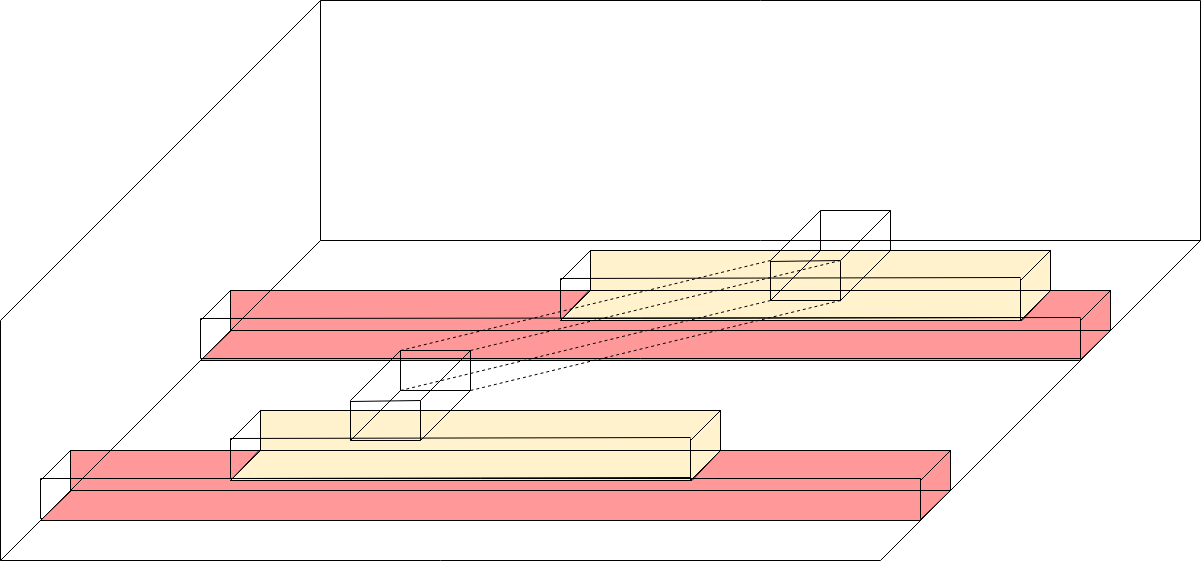
\includegraphics[scale=0.3]{img/Problembeschreibung/flamegraph_3D.png}
	\caption[3D Flammengraph]{Skizzierung eines dreidimensionalen Flammengraphs mit Nachrichtenaustausch}
	\label{fig:flamegraph_3D}
\end{figure}

% ----------------------------------------------------------------------------
